\documentclass[12pt]{article}
\usepackage[margin=1in]{geometry} 
\usepackage{amsmath,amsthm,amssymb,amsfonts,enumerate,listings,graphicx,epstopdf,siunitx}
\graphicspath{~/Documents/school/fall16/stat586/hw2}
 
\newcommand{\N}{\mathbb{N}}
\newcommand{\Z}{\mathbb{Z}}
 
\newenvironment{problem}[2][Problem]{\begin{trivlist}
\item[\hskip \labelsep {\bfseries #1}\hskip \labelsep {\bfseries #2.}]
  \vspace{1 cm}
}{\end{trivlist}}

\begin{document}
\title{Homework Set 2}
\author{Taylor Bodin}
\maketitle
 
\begin{problem}{2.29} 
\item let $p(m) \equiv E = E_1 \times E_2 \times \dots \times E_m  \rightarrow
  \prod_{i=1}^m n_i$ \\
  \begin{align*}
  p(1) &= E_1 \rightarrow n_1 \\
  p(2) &= E_1 \times E_2 \rightarrow n_1n_2 \\
  \dots \\
  p(k) &= E_1 \times E_2 \times \dots \times E_k \rightarrow \prod_{i=1}^k n_i
  & & \textrm{let the product equal } n_{\textrm{1 to k}} \\
  p(k+1) &= (E_1 \times \dots \times E_k) \times E_{k+1} \rightarrow 
  n_{\textrm{1 to k}}(n_{k+1}) = \prod_{i=1}^{k+1} n_i
  \end{align*}
\end{problem}

\begin{problem}{2.31} 
\item
  \begin{enumerate}[a.]
    \item % A
      \begin{align*}
        {{n}\choose{k}} &= {{n}\choose{n-k}} \\
        \frac{n!}{(n-k)!k!} &= \frac{n!}{(n-k)!(n-(n-k))!} \\
        &= \frac{n!}{(n-k)!(0+k)!} \\
        &= \frac{n!}{(n-k)!k!}
      \end{align*} 
    \item % B
     \begin{align*}
       \binom{n+1}{k+1} &= \binom{n}{k} + \binom{n}{k+1} \\
       \frac{(n+1)!}{(n+1-k-1)!(k+1)!} &= \frac{n!}{k!(n-k)!} + \frac{n!}{(k+1)!(n-k-1)!} \\
       \frac{(n+1)!}{(n-k)!(k+1)!} &= \frac{n!}{k!(n-k-1)!}\left(\frac{1}{n-k} + \frac{1}{k+1}\right) \\
       \frac{(n+1)!}{(n-k)!(k+1)!} &= \frac{n!}{k!(n-k-1)!}\left(\frac{k+1+n-k}{(n-k)(k+1)}\right) \\
       \frac{(n+1)!}{(n-k)!(k+1)!} &= \frac{n!}{k!(n-k-1)!}\left(\frac{n+1}{(n-k)(k+1)}\right) \\
       \frac{(n+1)!}{(n-k)!(k+1)!} &= \frac{(n+1)!}{(n-k)!(k+1)!} 
      \end{align*}
    \item %C
      \begin{align*}
        \sum_{k=0}^n \binom{n}{k} p^k q^{n-k} &= (p+q)^n & & \textrm{let } p = q = 1 \\
        \sum_{k=0}^n \binom{n}{k} 1^k 1^{n-k} &= (1+1)^n \\
        \sum_{k=0}^n \binom{n}{k} &= (2)^n
      \end{align*}
    \item %D
      \begin{align*}
        \sum_{k=0}^n \binom{n}{k} p^k q^{n-k} &= (p+q)^n & & \textrm{let } p = -1, q = 1 \\
        \sum_{k=0}^n \binom{n}{k}(-1)^k 1^{n-k} &= (-1+1)^n \\
        \sum_{k=0}^n \binom{n}{k}(-1)^k &= (0)^n \\
        \sum_{k=0}^n \binom{n}{k}(-1)^k &= 0 
      \end{align*}
    \item %E
      \begin{align*}
        \sum_{k=0}^n \frac{d}{dp}\left( \binom{n}{k} p^k q^{n-k}\right) &= \frac{d}{dp}\left((p+q)^n \right) \\
        \sum_{k=0}^n \binom{n}{k}k p^{k-1} q^{n-k} &= n(p+q)^{n-1} & & \textrm{let } p=q=1 \\
        \sum_{k=0}^n \binom{n}{k}k(1)^{k-1}(1)^{n-k} &= n(1+1)^{n-1} \\
        \sum_{k=0}^n \binom{n}{k}k &= n2^{n-1}
      \end{align*}
    \item %F
       \begin{align*}
        \sum_{k=0}^n \frac{d}{dp}\left( \binom{n}{k} p^k q^{n-k}\right) &= \frac{d}{dp}\left((p+q)^n \right) \\
        \sum_{k=0}^n \binom{n}{k}k p^{k-1} q^{n-k} &= n(p+q)^{n-1} & & \textrm{let } p=-1, q=1 \\
        \sum_{k=0}^n \binom{n}{k}k(-1)^{k-1}(1)^{n-k} &= n(-1+1)^{n-1} \\
        \sum_{k=0}^n \binom{n}{k}k(-1)^{k-1}(-1) &= 0(-1) \\
        \sum_{k=0}^n \binom{n}{k}k(-1)^{k} &= 0 
      \end{align*}
  \end{enumerate}
\end{problem}

\begin{problem}{2.33}
\item
  \begin{enumerate}[a.]
    \item %A
      $P(\textrm{1 Heart}) =  \frac{\binom{4}{1} \binom{48}{12}}{\binom{52}{13}} = \frac{9139}{20825} \approx .4388$
    \item %B
      $P(\textrm{7 or more of one suit}) 
      =  \frac{\binom{4}{1} \binom{13}{7} \binom{48}{12}}{\binom{52}{13}}
      = \frac{56628}{643195} \approx .0880$
    \item %C
      $P(\textrm{Void of one suit}) 
      =  \frac{\binom{4}{1} \binom{39}{13}}{\binom{52}{13}} 
      = \frac{17063919}{333515525} \approx .05116$
  \end{enumerate}
\end{problem}

\begin{problem}{2.35}
\item
  \begin{enumerate}[a.]
    \item %A
      $2^n$
    \item %B
      $\frac{\binom{3}{2} \binom{1}{1}}{2^3} = \frac{3}{8}$     
  \end{enumerate}
\end{problem}

\begin{problem}{2.37}
\item
  \begin{enumerate}[a.]
    \item %A
      $N_\textrm{codewords}(n) = \binom{n}{\frac{n}{2}}$, where N is even
    \item %B
      $N_\textrm{codewords}(8) = 70$ but $N_\textrm{codewords}(10) = 252 \therefore N = 10$
  \end{enumerate}
\end{problem}

\begin{problem}{2.39} %TODO
\item
  \begin{enumerate}[a.]
    \item %A
      $\frac{\binom{9}{3}}{2^9} = \frac{21}{128}$
    \item %B
      $\frac{2^9 - (\binom{9}{0} + \binom{9}{1} + \binom{9}{2}}{2^9} 
      =  \frac{233}{256} \approx .9102$
    \item %C TODO
     % $\frac{\binom{9}{3} \binom{6}{2} \binom{4}{1}}{2^9} possibly do the above, minus the sets with T<2 
  \end{enumerate}
\end{problem}

\begin{problem}{2.41} %TODO
 \item
   \begin{enumerate}[a.]
    \ item %A. 
      \begin{align*}
        \textrm{A} \cap \textrm{7,8,9,10,J,Q,K} &= 2 \binom{52}{4} \binom{51}{28} \\
        \textrm{Face Card, 10} \cap \textrm{8 or 9} &= 2 \binom{52}{16} \binom{51}{8} \\
        \textrm{Face Card, 10} \cap \textrm{Face Card, 10} &= 2 \binom{52}{16} \binom{51}{15} \\
        \textrm{9} \cap \textrm{9} &= \binom{52}{4} \binom{51}{3} \\
        P(\textrm{Hand} \geq 18) &= \frac{492}{2704}
       \end{align*}
    \item %B TODO 
      \begin{align*}
        \textrm{10 point} \cap \textrm{2,3,4,5,6,7} &= 2 \binom{52}{16} \binom{51}{12} \\
        \textrm{A} \cap \textrm{A,2,3,4,5,6} &= 2 \binom{52}{4} \binom{51}{23} \\
        \textrm{6} \cap \textrm{6,7,8,9} &= 2 \binom{52}{4} \binom{51}{15} \\
        \textrm{7} \cap \textrm{7,8,9} &= \binom{52}{4} \binom{51}{11} \\
        \textrm{8} \cap \textrm{8,9} &= \binom{52}{4} \binom{51}{7} \\
        P(\textrm{Hand} \geq 18) &= \frac{492}{2704}
      \end{align*}
  \end{enumerate}
\end{problem}

\begin{problem}{2.43}
\item
  \begin{enumerate}[a.]
    \item %A
      $\binom{52}{5}$
    \item %B
      $P(\textrm{Four Aces}) 
      = \frac{\binom{12}{1}\binom{4}{1}}{\binom{52}{5}}
      = \frac{1}{54145} \approx \num{1.847e-5}$
    \item %C
      $P(\textrm{Four of a Kind}) 
      = \frac{ \binom{13}{1} \binom{12}{1} \binom{4}{1}}{\binom{52}{5}}
      = \frac{1}{4165} \approx \num{2.401e-4}$
  \end{enumerate}
\end{problem}

\begin{problem}{2.45}
\item
  \begin{itemize}
    \item $P(A)$ is the probability of getting a computer from factory A
    \item $P(B)$ is the probability of getting a computer from factory B
    \item $P(D|A)$ is the probability of getting a defective computer given it came from factory A
    \item $P(D|B)$ is the probability of getting a defective computer given it came from factory B
  \end{itemize}
  \begin{align*}
    P(D|A) &= .15 \\
    P(D|B) &= .05 \\
    P(A) &= \frac{1000000}{1000000 + 150000} = \frac{20}{23} \\
    P(B) &= \frac{150000}{1000000 + 150000} = \frac{3}{23} \\
    P(D) &= P(D|A)P(A) + P(D|B)P(B) = .1370
  \end{align*}
\end{problem}

\begin{problem}{2.47}
\item
  \begin{enumerate}
    \item %Set Up 
      \begin{table}[!htpb]
        \centering
          \caption{Known Probabilities for 2.47}
          \label{probs_2_4}
            \begin{tabular}{lll}
              $P(0_{rx}|0_{tx}) = .9$  & $P(0_{rx}|1_{tx}) = .04$ & $P(0_{tx}) = .5$ \\
              $P(1_{rx}|0_{tx}) = .01$ & $P(1_{rx}|1_{tx}) = .8$  & $P(1_{tx}) = .5$ \\
              $P(E_{rx}|0_{tx}) = .09$ & $P(E_{rx}|1_{tx}) = .16$ & $P(E_{tx}) = 0$ 
            \end{tabular}
      \end{table}
    \item %A
      $P(E_{rx}) = P(E_{rx}|0_{tx})P(0_{tx}) + P(E_{rx}|1_{tx}) \approx .1250$
    \item %B
      \begin{align*}
        P(0_{tx}|E_{rx}) &= \frac{0_{tx} \cup E_{rx}}{P(E_{rx})} \\
        0_{tx} \cup E_{rx} &= P(E_{rx}|0_{tx})P(0_{tx}) \approx .0450 \\
        P(0_{tx}|E_{rx}) &\approx \frac{.0450}{.1250} \approx .3600 \\
      \end{align*}
    \item %C
      \begin{align*}
        P(P(1_{rx}|0_{tx})\cup P(0_{rx}|1_{tx})) &= P(1_{rx}|0_{tx}) + P(0_{rx}|1_{tx}) & & \textrm{Since these are mutually exclusive} \\
        P(P(1_{rx}|0_{tx})\cup P(0_{rx}|1_{tx})) &= .01 + .04 = .05 
      \end{align*}
  \end{enumerate}
\end{problem}

\begin{problem}{2.49}
\item
  \begin{table}[!htbp]
    \centering
    \begin{tabular}{llllllll}
      Year in School & $P(P)$ & $P(B)$ & $P(G)$ & $P(P|B)$ & $P(P|G)$ & $P(B|P)$ & $P(G|P)$ \\
      2nd grade      & .2774  & .45    & .55    & .25      & .30      & .4054    & .5946    \\
      4th grade      & .37    & .6     & .4     & .35      & .40      & .5676    & .4324    \\
      6th grade      & .5     & .52    & .48    & .5       & .5       & .52      & .48      \\
      8th grade      & .74    & .98    & .02    & .75      & .25      & .65      & .35     
    \end{tabular}
  \end{table}
\end{problem}

\begin{problem}{2.51}
\item
  \begin{enumerate}[a.]
    \item %A
      $P(x=5) = (1-\frac{1}{52})^{5-1} \frac{1}{52} \approx /num{1.779e-2}$
    \item %B
      $P(x\geq5) = (1-\frac{1}{52})^{5-1} \approx .9253$
    \item %C
      \begin{align*}
        P(x=5)
        &= (1-\frac{1}{52})(1-\frac{1}{51})(1-\frac{1}{50})(1-\frac{1}{49})(\frac{1}{48})
        &= \frac{1}{52} \\
        p(x\geq5) 
        &=(1-\frac{1}{52})(1-\frac{1}{51})(1-\frac{1}{50})(1-\frac{1}{49})
        &= \frac{12}{13}
      \end{align*}
  \end{enumerate}
\end{problem}

\begin{problem}{2.53}
\item
  $\frac{1}{2}$
\end{problem}

\begin{problem}{2.55}
\item
  \begin{enumerate}
    \item %A
      \begin{align*}
        P(A\cap \overline{B}) &= P(A)P(\overline{B}) \\
        P(A\cap \overline{B}) &= P(A)(1-P(B)) \\
        \frac{P(A\cap \overline{B})}{P{A}} &= P(\overline{B}) \\ 
        P(\overline{B}|P(A)) &= P(\overline{B}) \\ 
        P(\overline{B}) &= P(\overline{B}) 
      \end{align*}
    \item %B
      \begin{align*}
        P(\overline{A} \cap \overline{B}) &= P(\overline{A})P(\overline{B}) \\
        \frac{P(\overline{A} \cap \overline{B})}{P(\overline{B})} &= P(\overline{A}) \\
        P(\overline{A}|\overline{B}) &= P(\overline{A}) \\
        P(\overline{A}) &= P(\overline{A})
      \end{align*}
  \end{enumerate}
\end{problem}

\begin{problem}{2.57} %TODO
\item
  \begin{enumerate}[a.]
    \item %A

  \end{enumerate}
\end{problem}

\begin{problem}{2.59} %TODO
\item
\end{problem}

\begin{problem}{2.61} %TODO
\item
\end{problem}

\begin{problem}{2.63} %TODO
\item
\end{problem}

\begin{problem}{2.65} %TODO
\item
\end{problem}

\begin{problem}{2.67} %TODO
\item
\end{problem}

\begin{problem}{2.81} %TODO
\item
%  \lstinputlisting{problem_2_77.m} %}}}
\end{problem}


\begin{problem}{2.83} %TODO
\item
%  \begin{figure}[htpb]
%   \centering
%    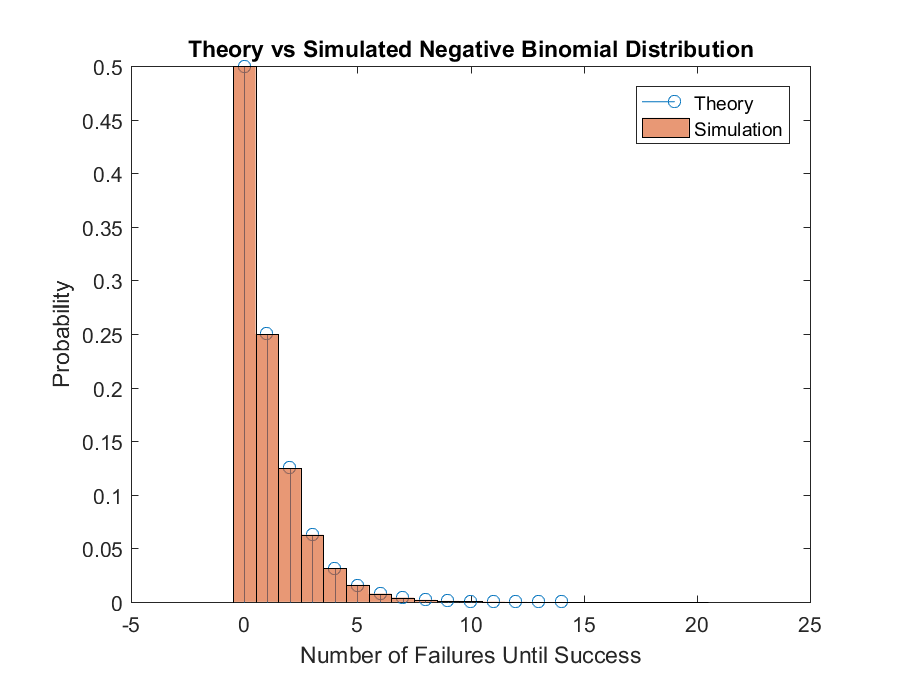
\includegraphics[scale=1]{fig_2_79.eps}
%    \caption{Problem 2.79, Simulation of the Negative Binomial Distribution}
%  \end{figure}%}}}
\end{problem}

\end{document}
